\documentclass[a4paper,10pt]{article}
\usepackage[utf8]{inputenc}
\usepackage[spanish]{babel}
\usepackage{graphicx}
\usepackage{epstopdf}
\usepackage{graphicx}
\usepackage{listings}
\usepackage{array}
\usepackage{hyperref}
\usepackage{tabularx}
\usepackage[margin=25mm]{geometry}

\title{Documento de Diseño de Air Guitar}
\author{Carlos Bergen Dyck \and Gustav Svensk}
\begin{document}

\renewcommand{\arraystretch}{1.5}
\maketitle
\begin{center}
        {\large Versión 0.1}
\end{center}
\newpage


\section{Prefacio}
\begin{tabular}{p{3cm} p{12cm}}
        & Este es el Documento de Diseño de Air Guitar, que consiste en
        producir sonido cuando se toca a su Air Guitar. \\
        \textbf{Alcance del documento} & El Documento de Diseño presenta las
        decisiones de diseño de Air Guitar. Describe los siguientes aspectos del
        sistema: arquitectura revisada, descripción de cada módulo, y diseño
        detallado de cada función incluyendo sus casos de prueba.\\
        \textbf{Documentos relacionados} & Documento de Requisitos de Air Guitar,
        versión 0.1, 6/11/2013. \\
        \textbf{Autor} & Carlos Bergen Dyck y Gustav Svensk \\
        \textbf{Lectores} & Este documento está dirigido principalmente a los
        desarrolladores del proyecto, pero es de interés de todos los
        interesados en como se implementa el proyecto. \\
        \textbf{Aprobación} & Este documento debe ser sometido a revisión de
        pares, pero no tiene una aprobación formal por alguien externo al equipo
        de desarrollo.
\end{tabular}

\section{Historia del Documento}
\begin{tabular}{|c|c|p{6cm}|p{4cm}|}
        \hline
        \textbf{Versión} & \textbf{Fecha} & \textbf{Explicación del cambio} &
        \textbf{Autor} \\ \hline
        0.1 & 25/11/2013 & Primer borrador & Carlos Bergen Dyck y Gustav Svensk \\
        \hline
\end{tabular}

\newpage
\tableofcontents

\listoftables

\listoffigures
\newpage

\section{Arquitectura Revisada del Sistema}
En el Documento de Requisitos de Nombre del Sistema se especificó su
arquitectura inicial. A la luz de un trabajo de diseño más detallado, aquí se
presenta la arquitectura definitiva, que incluye más detalle y posiblemente
algunos cambios.
\subsection{Diagrama de Contexto}
El diagrama de contexto se puede ver en figura~\ref{fig:contexto}.
\begin{figure}[h]
        \centering
        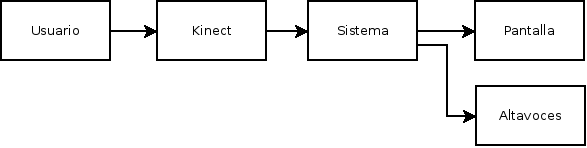
\includegraphics[width=0.8\textwidth]{../imagenes/diagrama_de_contexto.png}
        \caption{Diagrama de Contexto}
        \label{fig:contexto}
\end{figure}

\subsection{Diagrama de Arquitectura}
El diagrama de arquitectura se puede ver en figura~\ref{fig:arquitectura}
\begin{figure}[h]
        \centering
        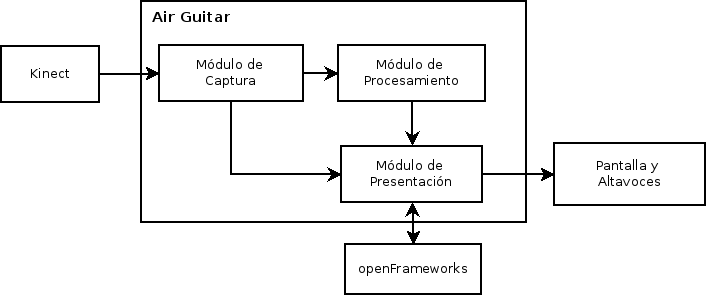
\includegraphics[width=0.8\textwidth]{../imagenes/diagrama_de_arquitectura.png}
        \caption{Diagrama de Arquitectura}
        \label{fig:arquitectura}
\end{figure}

\subsection{Enumeración de Módulos}
El cuadro~\ref{tab:modulos} muestra los módulos de la
figura~\ref{fig:arquitectura}. Por cada módulo se entrega un breve párrafo
descriptivo de su propósito, además de la sección en donde se especifica el
módulo en detalle.

\begin{table}[h]
        \centering
        \begin{tabularx}{\textwidth}{|p{3cm}| X |p{15mm}|}
                \hline
                \textbf{Módulo} & \textbf{Propósito} & \textbf{Sección} \\
                \hline
                Módulo de Captura (CAPT) & Obtener información del Kinect sobre el esqueleto del usuario. &\ref{sec:captura} \\
                \hline
                Módulo de Procesamiento (PROC) & Calcular el tono y volumen y ver si una nota fue tocada. &\ref{sec:procesamiento}\\
                \hline
                Módulo de Presentación (PRES) & Se encarga de dibujar las pantallas de la aplicación y la guitarra asi como reproducir los sonidos de las notas tocadas. &\ref{sec:presentacion}\\
                \hline
        \end{tabularx}
        \caption{Módulos de la arquitectura del sistema}
        \label{tab:modulos}
\end{table}

\subsection{Matriz de Requisitos Funcionales y Módulos}
En tabla~\ref{tab:req_func} están los requisitos funcionales del sistema y en
tabla~\ref{tab:matriz} la matriz de requisitos funcionales y módulos.
\begin{table}[hpb]
        \centering
        \begin{tabularx}{0.8\textwidth}{p{8mm} X}
                \textbf{RF1} & Obtener la posición de las manos y la caldera \\
                \textbf{RF2} & Obtener la velocidad de la mano derecha \\
                \textbf{RF3} & Calcular tono y volumen en base a la posición y velocidad de las manos \\
                \textbf{RF4} & Reproducir sonido a base al tono y volumen \\
                \textbf{RF5} & Proyectar modelo 3D de guitarra \\
        \end{tabularx}
        \caption{Requisitos Funcionales}
        \label{tab:req_func}
\end{table}
\begin{table}[hpb]
        \centering
        \begin{tabular}{|p{8mm}|c|c|c|}
                \hline
                & \textbf{CAPT} & \textbf{PROC} & \textbf{PRES} \\
                \hline
                \textbf{RF1} & X & & \\
                \hline
                \textbf{RF2} & & X & \\
                \hline
                \textbf{RF3} & & X & \\
                \hline
                \textbf{RF4} & & & X \\
                \hline
                \textbf{RF5} & & & X \\
                \hline
        \end{tabular}
        \caption{Matriz de Requisitos Funcionales y Módulos}
        \label{tab:matriz}
\end{table}
\section{Módulo de Captura}
\label{sec:captura}
\subsection{Definición de Módulo}
\begin{tabularx}{\textwidth}{p{25mm} X}
        \textbf{Propósito} & Obtener información del Kinect sobre el esqueleto del usuario.\\
        \textbf{Alcance} & Obtiene la posición de las manos y de la cadera.\\
        \textbf{Dependencias} & Depende de la información recibida del Kinect.\\
        \textbf{Supuestos} & Tener Kinect. \\
        \textbf{Restricciones} & Usar PC con Windows. Estar a una distancia aceptable del Kinect y que exista una iluminación adecuada.\\
        \textbf{Estructura General} & Obtiene las posiciones de las manos y la cadera y entrega estos puntos al modulo de procesamiento.\\
\end{tabularx}
\subsection{Declaraciones Públicas}
Esta sección enumera constantes, tipos y variables del módulo, visibles para
otros módulos.
\subsubsection{Constantes Públicas}
\begin{tabular}{| p{30mm} | p{10cm} |}
        \hline
        \textbf{Nombre de la \mbox{constante}} & \textbf{Descripción} \\
        \hline
         & \\
        \hline
\end{tabular}
                

\subsubsection{Tipos de Datos Públicos}
\begin{tabular}{| p{30mm} | p{10cm} |}
        \hline
        \textbf{Nombre del \mbox{tipo}} & \textbf{Descripción} \\
        \hline
         & \\
        \hline
\end{tabular}
\subsubsection{Variables Públicos}
\begin{tabular}{| p{30mm} | p{10cm} |}
        \hline
        \textbf{Nombre de la \mbox{variable}} & \textbf{Descripción} \\
        \hline
         & \\
        \hline
\end{tabular}
\subsection{Funciones Públicas}
Las siguientes funciones son accesibles desde otros módulos. Otros módulos
tienen acceso a la funcionalidad de este módulo mediante estas funciones.
~\\

\begin{tabular}{| p{30mm} | p{10cm} |}
        \hline
        \textbf{Nombre de la \mbox{función}} & \textbf{Descripción breve} \\
        \hline
         & \\
        \hline
\end{tabular}
\subsection{Estructuras de Datos}
\subsection{Funciones Privadas}
Las siguientes funciones auxiliares son privadas de este módulo; otros módulos
no las pueden usar.
~\\

\begin{tabular}{| p{30mm} | p{10cm} |}
        \hline
        \textbf{Nombre de la \mbox{función}} & \textbf{Descripción breve} \\
        \hline
         & \\
        \hline
\end{tabular}
\subsection{Diseño Detallado de las Funciones}
\subsubsection{Función 1}
\begin{tabularx}{\textwidth}{p{25mm} X}
        \textbf{Propósito} & \\
        \textbf{Dependencias} & \\
        \textbf{Prototipo} & \\
        \textbf{Parámetro} & \textbf{Explicación} \\
        \begin{tabular}{p{2cm} l}
                Parámetro 1 & \\
        \end{tabular}

        \textbf{Retorno} & \\
        \textbf{Proceso} & Pseudocodigo \\
\end{tabularx}


\section{Módulo de Procesamiento}
\label{sec:procesamiento}
\subsection{Definición de Módulo}
\begin{tabularx}{\textwidth}{p{25mm} X}
        \textbf{Propósito} & Calcular el tono y volumen y ver si una nota fue tocada.\\
        \textbf{Alcance} & Calcula el tono basado en la distancia de la mano izquierda y la cadera. Calcula el volumen basado en la velocidad de la mano derecha y ve si una nota fue tocada si la mano derecha se encuentra sobre un área predefinida.\\
        \textbf{Dependencias} & Depende del modulo de captura.\\
        \textbf{Supuestos} & Un funcionamiento correcto del modulo de captura.\\
        \textbf{Restricciones} & Existira un rango de tonos disponibles para tocar y tendra un limite de volumen.\\
        \textbf{Estructura General} & Recibe los puntos obtenidos del modulo de captura. Entrega el tono y volumen de la nota actual y si esta debe ser reproducida. Entrega la posición donde debe ser proyectada la guitarra. \\
\end{tabularx}
\subsection{Declaraciones Públicas}
Esta sección enumera constantes, tipos y variables del módulo, visibles para
otros módulos.
\subsubsection{Constantes Públicas}
\begin{tabular}{| p{30mm} | p{10cm} |}
        \hline
        \textbf{Nombre de la \mbox{constante}} & \textbf{Descripción} \\
        \hline
         & \\
        \hline
\end{tabular}
                

\subsubsection{Tipos de Datos Públicos}
\begin{tabular}{| p{30mm} | p{10cm} |}
        \hline
        \textbf{Nombre del \mbox{tipo}} & \textbf{Descripción} \\
        \hline
         & \\
        \hline
\end{tabular}
\subsubsection{Variables Públicos}
\begin{tabular}{| p{30mm} | p{10cm} |}
        \hline
        \textbf{Nombre de la \mbox{variable}} & \textbf{Descripción} \\
        \hline
         & \\
        \hline
\end{tabular}
\subsection{Funciones Públicas}
Las siguientes funciones son accesibles desde otros módulos. Otros módulos
tienen acceso a la funcionalidad de este módulo mediante estas funciones.
~\\

\begin{tabular}{| p{30mm} | p{10cm} |}
        \hline
        \textbf{Nombre de la \mbox{función}} & \textbf{Descripción breve} \\
        \hline
         & \\
        \hline
\end{tabular}
\subsection{Estructuras de Datos}
\subsection{Funciones Privadas}
Las siguientes funciones auxiliares son privadas de este módulo; otros módulos
no las pueden usar.
~\\

\begin{tabular}{| p{30mm} | p{10cm} |}
        \hline
        \textbf{Nombre de la \mbox{función}} & \textbf{Descripción breve} \\
        \hline
         & \\
        \hline
\end{tabular}
\subsection{Diseño Detallado de las Funciones}
\subsubsection{Función 1}
\begin{tabularx}{\textwidth}{p{25mm} X}
        \textbf{Propósito} & \\
        \textbf{Dependencias} & \\
        \textbf{Prototipo} & \\
        \textbf{Parámetro} & \textbf{Explicación} \\
        \begin{tabular}{p{2cm} l}
                Parámetro 1 & \\
        \end{tabular}

        \textbf{Retorno} & \\
        \textbf{Proceso} & Pseudocodigo \\
\end{tabularx}


\section{Módulo de Presentación}
\label{sec:presentacion}
\subsection{Definición de Módulo}
\begin{tabularx}{\textwidth}{p{25mm} X}
        \textbf{Propósito} & Se encarga de dibujar las pantallas de la aplicación y la guitarra asi como reproducir los sonidos de las notas tocadas.\\
        \textbf{Alcance} & Reproduce el sonido correspondiente a la nota calculada y proyecta un modelo 3D de una guitarra sobre el usuario.\\
        \textbf{Dependencias} & Depende del modulo de procesamiento.\\
        \textbf{Supuestos} & Tener una tarjeta gráfica apropiada asi como una tarjeta de sonido.\\
        \textbf{Restricciones} & Reproducira los sonidos correspondientes definidos anteriormente.\\
        \textbf{Estructura General} & Recibe la posición de la guitarra, el tono y volumen de la nota y si esta fue tocada. Dibuja en la pantalla la imagen del usuario con un modelo 3D de una guitarra proyectada y reproduce el sonido apropiado.\\
\end{tabularx}
\subsection{Declaraciones Públicas}
Esta sección enumera constantes, tipos y variables del módulo, visibles para
otros módulos.
\subsubsection{Constantes Públicas}
\begin{tabular}{| p{30mm} | p{10cm} |}
        \hline
        \textbf{Nombre de la \mbox{constante}} & \textbf{Descripción} \\
        \hline
         & \\
        \hline
\end{tabular}
                

\subsubsection{Tipos de Datos Públicos}
\begin{tabular}{| p{30mm} | p{10cm} |}
        \hline
        \textbf{Nombre del \mbox{tipo}} & \textbf{Descripción} \\
        \hline
         & \\
        \hline
\end{tabular}
\subsubsection{Variables Públicos}
\begin{tabular}{| p{30mm} | p{10cm} |}
        \hline
        \textbf{Nombre de la \mbox{variable}} & \textbf{Descripción} \\
        \hline
         & \\
        \hline
\end{tabular}
\subsection{Funciones Públicas}
Las siguientes funciones son accesibles desde otros módulos. Otros módulos
tienen acceso a la funcionalidad de este módulo mediante estas funciones.
~\\

\begin{tabular}{| p{30mm} | p{10cm} |}
        \hline
        \textbf{Nombre de la \mbox{función}} & \textbf{Descripción breve} \\
        \hline
         & \\
        \hline
\end{tabular}
\subsection{Estructuras de Datos}
\subsection{Funciones Privadas}
Las siguientes funciones auxiliares son privadas de este módulo; otros módulos
no las pueden usar.
~\\

\begin{tabular}{| p{30mm} | p{10cm} |}
        \hline
        \textbf{Nombre de la \mbox{función}} & \textbf{Descripción breve} \\
        \hline
         & \\
        \hline
\end{tabular}
\subsection{Diseño Detallado de las Funciones}
\subsubsection{Función 1}
\begin{tabularx}{\textwidth}{p{25mm} X}
        \textbf{Propósito} & \\
        \textbf{Dependencias} & \\
        \textbf{Prototipo} & \\
        \textbf{Parámetro} & \textbf{Explicación} \\
        \begin{tabular}{p{2cm} l}
                Parámetro 1 & \\
        \end{tabular}

        \textbf{Retorno} & \\
        \textbf{Proceso} & Pseudocodigo \\
\end{tabularx}

\newpage
\section{Diseño de Interfaces}
\subsection{Modelo de Navegación}
El modelo de navegación es muy simple porque sólo hay una interfaz
(figura~\ref{fig:navegacion}).

\begin{figure}[hb]
        \centering
        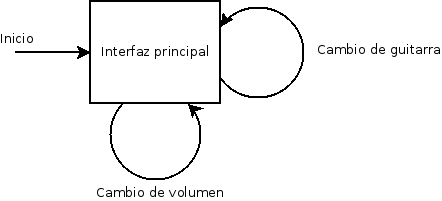
\includegraphics[width=0.7\textwidth]{../imagenes/modelo_de_navegacion.png}
        \caption{Modelo de Navegación}
        \label{fig:navegacion}
\end{figure}
\subsection{Prototipos de Interfaces Usuarias}
\subsubsection{Prototipo Interfaz Principal}
En figura~\ref{fig:ui} se puede ver la interfaz principal. En el programa final
el fondo será el usuario con una guitara sobrepuesta.

\begin{tabularx}{\textwidth}{X X X X}
        \textbf{Evento} & \textbf{Interacción} & \textbf{Acción} & \textbf{Objeto afectado} \\
        Cambio de volumen & El usuario mueve el slider ``Volumen'' & Se
        modifica el volumen & Módulo de Presentación \\
        Cambio de guitarra & El usuario aprieta el botón ``Acustic'' o
        ``Electric'' & Se cambia el modelo de la guitarra y el sonido & Módulo
        de Presentación \\


\end{tabularx}
\begin{figure}[hb]
        \centering
        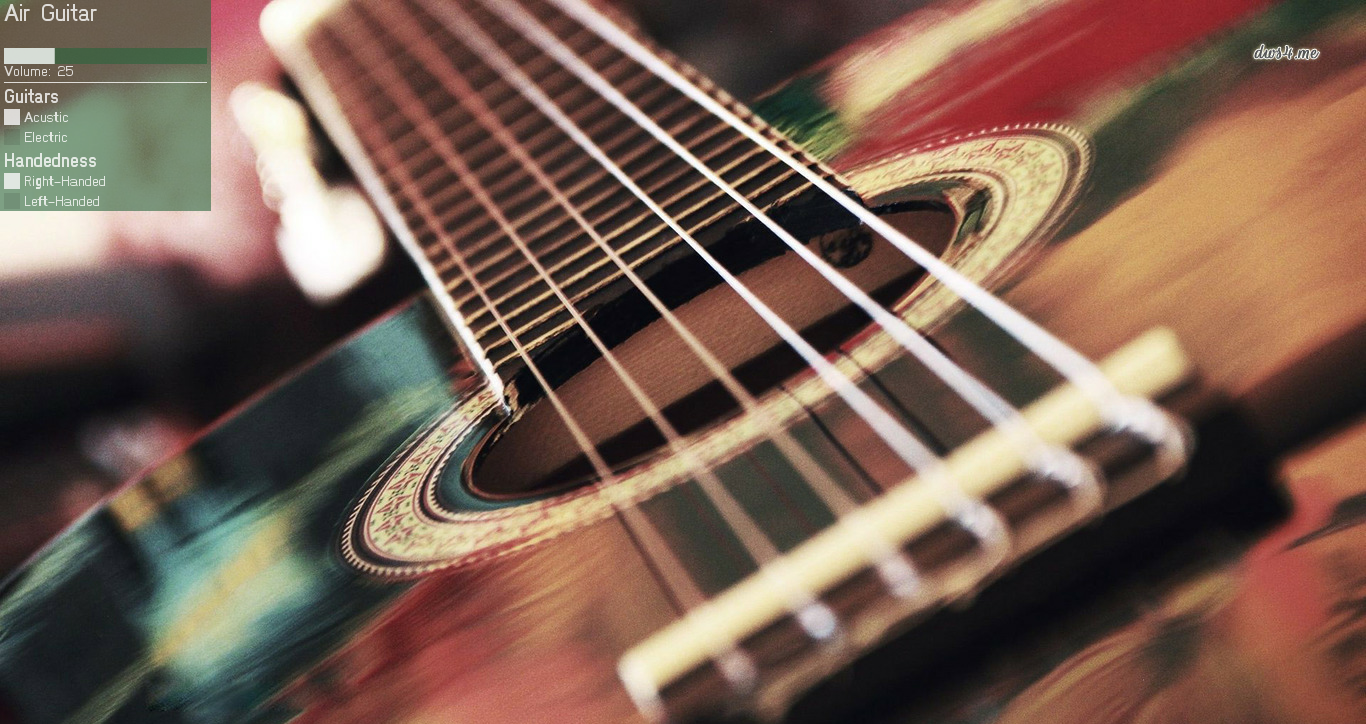
\includegraphics[width=\textwidth]{../imagenes/ui.png}
        \caption{La interfaz principal}
        \label{fig:ui}
\end{figure}
\newpage
% \appendix 

% \addcontentsline{toc}{section}{Referencias}
% \begin{thebibliography}{99}
% \bibitem{depth_range}\url{http://msdn.microsoft.com/en-us/library/hh973078.aspx#Depth_Ranges} \\
%         Microsoft Developer Network, 05 Nov 2013
% \bibitem{air_guitar}\url{https://en.wikipedia.org/wiki/Air_guitar#Contests} \\
%         Wikipedia, 05 Nov 2013
% \bibitem{kinect_spec}\url{http://msdn.microsoft.com/en-us/library/jj131033.aspx} \\
%         Microsoft Developer Network, 05 Nov 2013
% \bibitem{kinect_release}\url{http://en.wikipedia.org/wiki/Kinect#History} \\
%         Wikipedia, 05 Nov 2013
% \bibitem{sdk}\url{http://msdn.microsoft.com/en-us/library/hh855347.aspx} \\
%         Microsoft Developer Network, 05 Nov 2013
% \bibitem{kinect_new}\url{http://blogs.msdn.com/b/kinectforwindows/archive/2013/09/16/updated-sdk-with-html5-kinect-fusion-improvements-and-more.aspx} \\
%         Kinect for Windows Blog, 05 Noc 2013
% \end{thebibliography}

\end{document} 
%%% Local Variables: %%% mode: latex %%% TeX-master: t %%% End:
